\chapter{Results} \label{ch:results}

In this chapter, we analyze models regarding their feature distribution and algorithms regarding their performance.
Furthermore, we investigate which model features influence on the performance of the algorithms.

%Regarding runtime a lot of stuff may change. Iterations wont change as long as we use the same deterministic algorithms, so its a more stable metric.

%Various studies we have made, knit into a nice purple string and story. Here might appear:
%Maybe it would also be cool to show preformance differences in real case studies in comparison to the randomly generated models and make conclusions Ideally:
%\textcolor{purple}{We did previously not have enough models to see behaviour XYZ but now we can.}

\section{Experimental Setup}
Various algorithms we consider were already implemented in PRISM-games~\cite{prismgames3}.
We needed to extend PRISM-games by the algorithms $\LPSI$, $\TLPSI$, and $\TOPAlg$.
Moreover, for $\TOPAlg$ we added precise Markov chain solving, which was not present in PRISM-games before, and extended the strategy iteration (which was implemented in~\cite{gandalf20}) to use this precise solving.
Our code is available in the GitHub repository \url{https://github.com/ga67vib/Algorithms-For-Stochastic-Games}.

\subsubsection*{Technical details}
We conducted the experiments on a server with 64 GB of RAM and a 3.60GHz Intel CPU running Manjaro Linux. %Intel (R) Xeon(R) W-2123 CPU.
We always use a precision of $\varepsilon=10^{-6}$. The timeout was set to 15 minutes for all models. 
The memory limit for every experiment was 6 GB.

\section{Model Analysis Results}

First, we want to learn about the feature distribution of the real case studies we have. 
For this we use in Figure \ref{fig:Real_FeatureDistribution} a box plot for each feature.
In each graph, the distribution of the values of one separate feature in all real case studies is visualized. 
The orange line marks the median of a feature in all models and the green triangle marks the average.
The bounds of the boxes mark the 25 and 75 percentile, and the lines extended by the whiskers mark the 10 and 90 percentile.
%\textcolor{red}{Not sure about the 10 and 90 percentiles}
Dots outside of whiskers represent outliers.
The relative number of probabilistic actions for example is between around $15\%$ and $45\%$ in half of the models.
In half of the models, more than $20\%$ of actions are probabilistic.
\textcolor{purple}{Most likely I may move all the features into the appendix and only highlight 5-10 cool features.}
\begin{figure}[t]
    \centering
    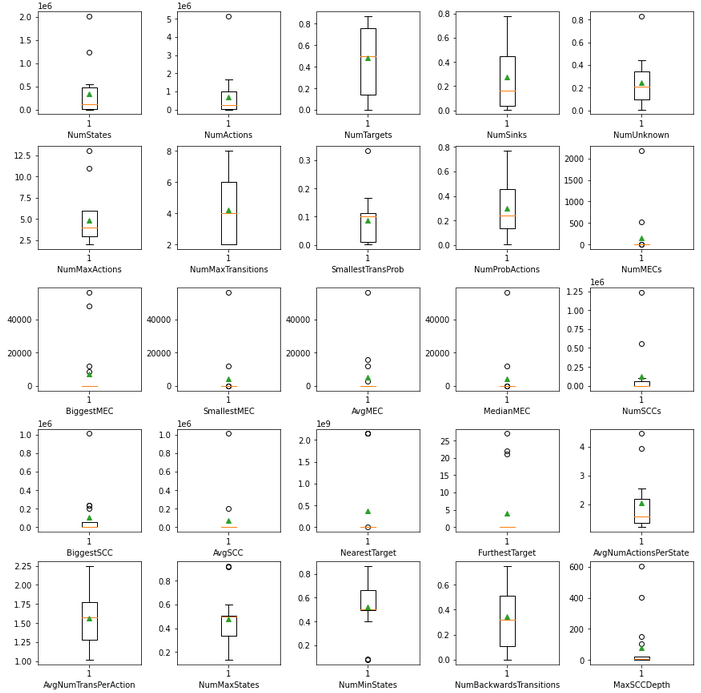
\includegraphics[width=1\textwidth]{figures/Real_FeatureDistribution.png}
    \caption[Feature Distribution of the case studies]{
        Box plot of the feature distribution of the real case studies.
    }
    \label{fig:Real_FeatureDistribution}
\end{figure}
What we can read from the box plot is this:
\begin{itemize}
    \item Models have around 2 actions per state and 1.5 Transitions per action
    \item On average, 80\% of the states of the models are trivial, and their value can be computed with simple graph algorithms 
    \item Generally, the number of states is evenly split to Maximizer and Minimizer
    \item Usually, around 70 to 85\% of all actions are deterministic
    \item Most models do not contain end components
\end{itemize}

By furthermore printing the maximal and minimal occurring values of each feature we obtain that the smallest occurring positive transition probability is 0.001.

With this information, we can draw conclusions about which structural cases do not appear in the real case studies. 
None of the models contain these cases:
\begin{itemize}
    \item Models with numerous actions per state
    \item Models with numerous Transitions per action
    \item Models with very small transition probabilities like 1e-6
\end{itemize}

We can also use box plots to evaluate for which features our random generation procedure from Chapter \ref{ch:randomGen} is biased.
We do so in Figure \ref{fig:Random_FeatureDistribution}.
\begin{figure}[t]
    \centering
    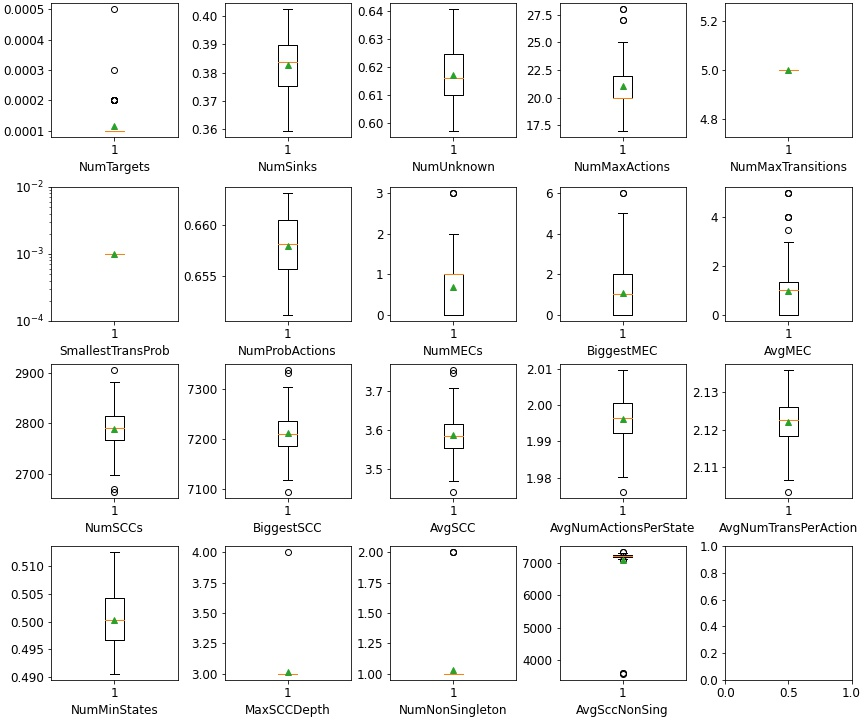
\includegraphics[width=1\textwidth]{figures/RandomRandom_FeatureDistribution.png}
    \caption[Feature Distribution of random models]{
        Feature Distribution of random models
    }
    \label{fig:Random_FeatureDistribution}
\end{figure}

The biases we read from this plot are:
\begin{itemize}
    \item On average, 70\% of the states of the models can be computed by trivial graph algorithms. NumSinks shows that almost all known states are sinks.
            This is because we use the forceUnknown switch, which guarantees that there is only one goal state. 
            However, there can be multiple sinks because of end components containing only minimizer states. 
            In this case, once the token is inside the end component the Minimizer can pick a strategy such that the token never leaves and thus can never reach the target.
    \item As mentioned in Chapter \ref{ch:randomGen}, our procedure generates models with a tendency to have few actions per state and few transitions per action.
    \item NumMecs shows that are usually at most three MECs per model
    and NumNonSingleton shows that in almost all cases there is only one strongly connected component.
        This is because we uniformly randomize where the transition may lead. Thus, it is likely that big MECs and SCCs are formed. 
    \item \textcolor{purple}{The rest of the current image is very dependent on the parameters we set, so it is pointless talking about it.
          Or we could use it as an example.}
          \textcolor{red}{However, I should create 100 models with the same parameters and then see their feature distribution of non-set features. Do this once I have reimplemented random generation}
\end{itemize}

Our random generation procedure introduces a bias towards various properties like for example, the number of SCCs or the average number of transitions per Action. 
To regain control over these properties, we can use other guidelines as described in Section \ref{sec:guidelines}.
\textcolor{red}{Show the Figure of SCC FeatureDistribution for RandomSCC benches.}
However, when comparing the feature distributions of the real case studies and the distributions of the models generated by Algorithm \ref{algo:randomRandom},
they have similar biases for many features. Both Benchmarks tend to have few big SCCs, few actions per state, and few transitions per action.
Thus, our procedure is capable of recreating models that have in various regards a similar structure to the currently available real case studies. 

\section{Algorithm Comparison Results}

In this section, we compare the Algorithms introduced in Section \ref{sec:SGAlgos} on real case studies, handcrafted examples, and our randomly generated models to both evaluate the 
performance of the algorithms relative to each other and find correlations between model feature values and algorithm performance.

\subsubsection*{Case studies}
We consider case studies from three different sources: 
(i) all real case studies that were already used in~\cite{gandalf20}, which are mainly from the PRISM benchmark suite~\cite{PRISMben}. We omit models that are already solved by pre-computations.
(ii) several handcrafted corner case models: haddad-monmege (an adversarial for value iteration from~\cite{haddadmonmege}), BigMec (a single big MEC), and MulMec (a long chain of many small MECs), the latter two both being from~\cite{gandalf}.
(iii) randomly generated models generated by Algorithm \ref{algo:randomRandom} and our additional guidelines from Subsection \ref{sec:guidelines}.
\textcolor{red}{Here we should state the exact parameters we have used for our models. States are 1000 to 10000.}


\textcolor{red}{Another way to write this section is to start out with the star-graph, take each clue and build a string from there.}

First, we provide a general overview of the performance of all algorithms on our benchmarking set in Figure \ref{fig:AlgoPerformance}.
The plots depict the number of solved benchmarks (x-axis) and the time it took to solve them (y-axis). 
For each algorithm, the benchmarks are sorted ascending by verification time. A line stops when no further benchmarks could be solved.
Intuitively, the further to the bottom right a plot is, the better; where going right (solving benchmarks) is more relevant.
The legend on the right is sorted by the performance of the algorithms.
Note that this plot has to be interpreted with care, as it greatly depends on the selection of benchmarks.
\textcolor{purple}{Should make the both plots in jupyter next to each other. This gives the best quality screenshots. If not possible then at least make the height smaller}
\begin{figure}
    \centering
    \subfloat[\centering Performance Overview on real case studies]{{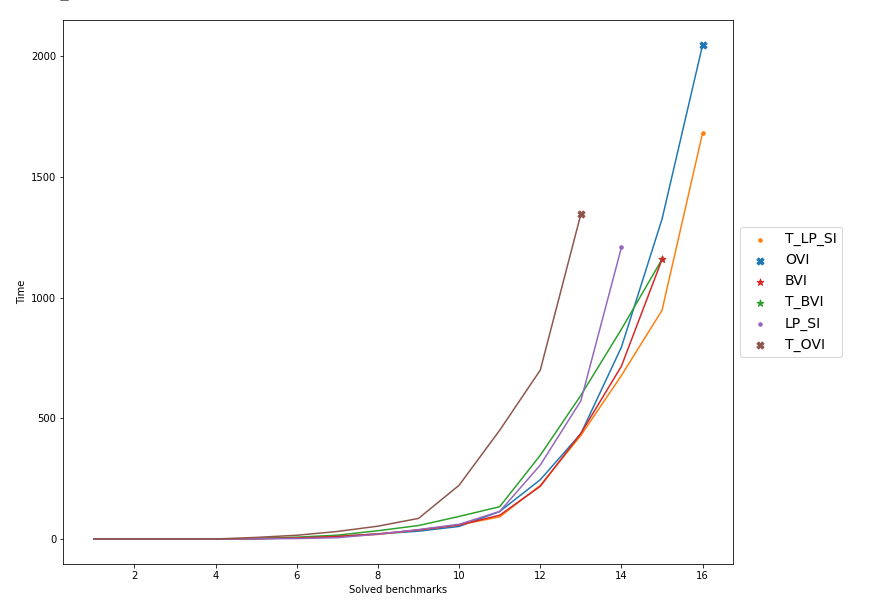
\includegraphics[width=0.8\textwidth]{figures/Real_AlgoPerformance.png} }}%
    \qquad
    \subfloat[\centering Performance Overview on randomly generated models]{{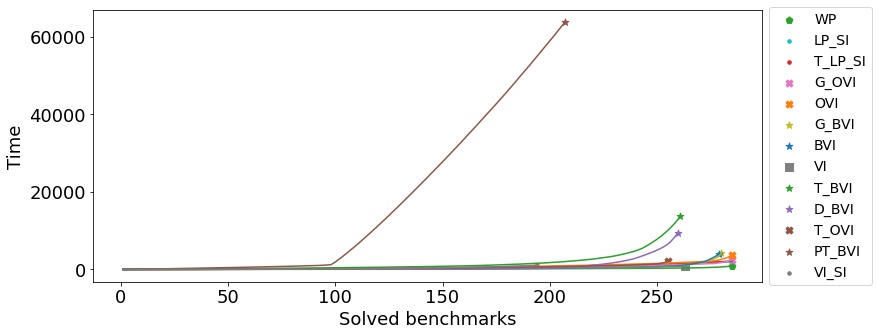
\includegraphics[width=0.8\textwidth]{figures/RandomRandom_AlgoPerformance.png} }}%
    \caption[Overview of Algorithm Performance]{Overview of Algorithm Performance}%
    \label{fig:AlgoPerformance}
\end{figure}

%For value-iteration-based algorithms, we provide the same graph with the number of iterations required to solve the models on the y-axis in Figure
%\ref{fig:AlgoPerformanceIters} \textcolor{red}{Add star-graph for iterations}.

We read several clues from Figure \ref{fig:AlgoPerformance}. 
$\WP$, $\OVI$, and $\TLPSI$ seem to be the most performant algorithms for our benchmarks. 
Also, Optimizations mentioned in Subsection \ref{subsec:optimizations} do not seem to have in general a positive impact on their baseline algorithms.

We split our analysis into three subtopics: 
First, we compare the three value-iteration-based algorithms with guarantees $\OVI$, $\WP$, and $\BVI$. 
Then, we analyze the impact of the optimizations from Subsection \ref{subsec:optimizations} on their respective baseline algorithms.
Lastly, we investigate the performance of $\LPSI$ and $\TLPSI$ in comparison to value-iteration-based algorithms.


\subsection{$\BVI$ vs $\OVI$ vs $\WP$}
We can read from Figure \ref{fig:AlgoPerformance} that WP is the fastest to solve the problems on both random-generated models and real case studies.
To see whether this is the case for all models or only accumulated, we consider the scatter plot in Figure \ref{fig:WPvsBVIandOVIonRandomRandom}.
Each point in the graph is a model. The x-axis marks the time $\WP$ requires to solve the stochastic game, and the y-axis marks the respective time $\BVI$ or $\OVI$.
The two lines next to the diagonal mark the case that $\WP$ is twice as fast as $\BVI$ / $\OVI$s or half as fast.

\begin{figure}[t]
    \centering
    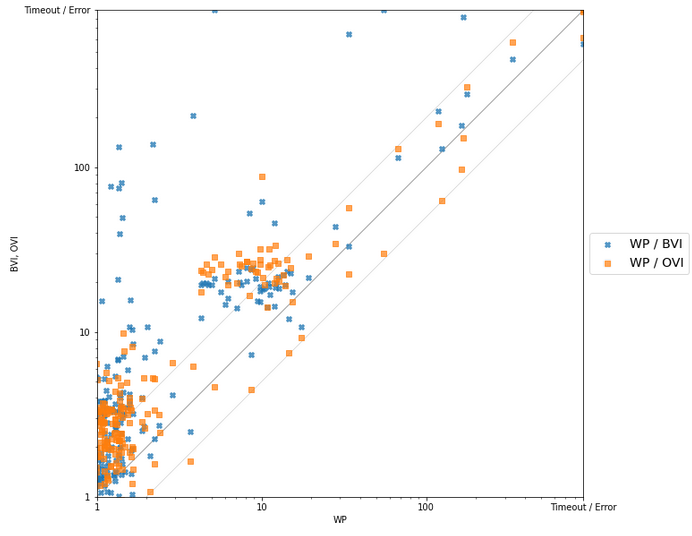
\includegraphics[width=1\textwidth]{figures/WPvsBVIandOVIonAll.png}
    \caption[$\WP$ compared to $\BVI$ and $\OVI$ on time necessary to solve models]{
        $\WP$ compared to $\BVI$ and $\OVI$ on time necessary to solve models
    }
    \label{fig:WPvsBVIandOVIonRandomRandom}
\end{figure}

$\WP$ is usually faster than $\BVI$ and $\OVI$ and never requires more than twice as long.
Next, we are interested in whether there is a correlation between structural properties and $\WP$ being better or worse than the other two.
To inspect the cases where $\WP$ is better than $\OVI$ or the other way around, we plot the feature of the models where one algorithm was at least
1.5 times faster than the other one. Figure \ref{fig:WPvsOVIon1DFeatureScatter} visualizes these cases. 
The red dots mark models where $\OVI$ is at least 1.5 times faster than $\WP$, and the green dots mark models where $\WP$ is at least 1.5 times faster than $\OVI$.
The x-axis displays the range of values that occur for the feature. 
If the dots are clustered for a feature, either one algorithm was only faster if the model had this kind of structural composition, 
or there are only discrete values available for the feature. For example, the number of states is mostly discrete because the random models depend on an input parameter.

\begin{figure}[t]
    \centering
    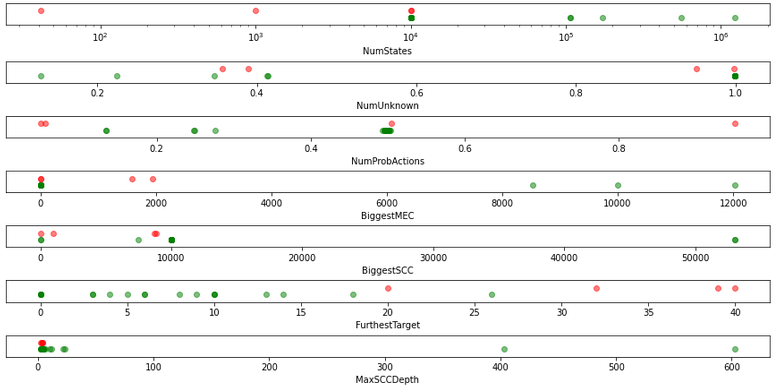
\includegraphics[width=1\textwidth]{figures/WPvsOVIon1DFeatureScatter.png}
    \caption[$\WP$ compared to $\OVI$]{
        The red dots mark models where $\OVI$ is at least 1.5 times faster than $\WP$, and the green dots mark models where $\WP$ is at least 1.5 times faster than $\OVI$.
        The x-axis displays the range of values that occur for the feature. 
        If the dots are clustered for a feature, either one algorithm was only faster if the model had this kind of structural composition, 
        or there are only discrete values available for the feature. For example, the number of states is mostly discrete because the random models depend on an input parameter.
    }
    \label{fig:WPvsOVIon1DFeatureScatter}
\end{figure}

According to Figure \ref{fig:WPvsOVIon1DFeatureScatter}, $\WP$ was better than $\OVI$ if the model had more states, had big MECs and big SCCs.
$\OVI$ seems to be better if the furthest target is far away from the initial state, but since we cannot tie this to any structural significant property,
it may also be noise. If this interpretation is correct, $\WP$ should become even better than $\OVI$ if we use larger models.

The same plot for $\WP$ and $\BVI$ is harder to interpret since there are only two cases where $\BVI$ is 1.5 times faster than $\OVI$, and 40 cases
for the opposite event. Thus, we conclude that $\WP$ is in all more performant on our benchmarks than $\BVI$ regarding runtime. 
\textcolor{blue}{The two cases where BVI is better are quite noisy, so it is not worth including the Figure in my Opinion.
But I have added it in case you think it is interesting. It is Figure \ref{fig:WPvsBVIon1DFeatureScatter}}

\begin{figure}[t]
    \centering
    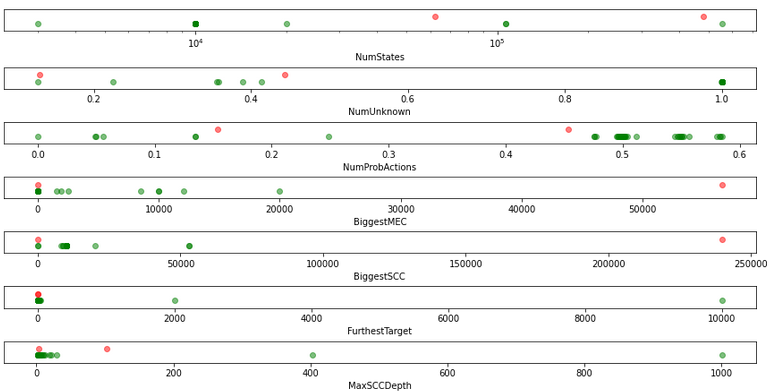
\includegraphics[width=1\textwidth]{figures/WPvsBVIon1DFeatureScatter.png}
    \caption[$\WP$ compared to $\BVI$]{
        Comparing cases where $\WP$ is better than $\BVI$ (green) and $\BVI$ is better than $\WP$ (red) 
        and plotting the corresponding feature values of the models.
    }
    \label{fig:WPvsBVIon1DFeatureScatter}
\end{figure}


However, time is not the best measure we can use to compare value-iteration-based approaches. 
This is because time may be very dependent on optimization in the code. 
For value-iteration-based algorithms, we can also compare the iteration count, which depends only on the algorithm itself.
Thus, we provide an analogous scatter plot in Figure \textcolor{red}{ITERATION SCATTER} where the axes mark the iterations required to solve a model.

\textcolor{red}{Next, add big models to confirm that the thesis you set up also holds for big models. 
There you can also say that although $\OVI$ looks promising in the small models, in the big models it may fall behind $\BVI$.}

\subsection{Analyzing the Optimizations}

$\mathbf{Gauss-Seidel} \ \BVI$:

\textcolor{purple}{Generally fewer iterations, but matrix operations of vanilla is faster than state-by-state.
Can sometimes be worse even for iterations due to unlucky SCCs based on lower bound. Then the upperbound can fall behind the vanilla upperbound
GS-bvi along topological enumeration of states could not improve our results. Show some graphs of how it did not improve?}

$\mathbf{D} \ \BVI$:

\textcolor{purple}{Show time scatter, say two sentences (no huge improvement), go on}

$\mathbf{T} \ \BVI, \OVI$ and $\LPSI$:

As the scatter plot \textcolor{red}{Ref to scatter plot TLPSI vs LPSI} shows,
the topological addition for strategy iteration with linear programming in the real case studies and random models does 
neither in- nor decrease the performance of the algorithm considerably.
However, most models have very few SCCs, so the topological optimization does not contribute much.
The data point where $\TLPSI$ is significantly faster is on the real case study "dice", where every state is an SCC on its own.
This is obviously the best-case scenario for topological algorithms.
\textcolor{red}{Show Scatter.
Explain why $\OVI$ and $\BVI$ do not scale that well (explained in Gandalf Paper)}

$\TOPAlg \ \BVI$:

$\TOPAlg$ seems to perform worse than $\BVI$ in general. This is because we solve the DTMCs with exact methods, 
\textcolor{red}{Scatter BVI vs TOP}
requiring a matrix inversion, which is $\mathcal{O}(n^{2})$-operation, where n is the number of states in the SCC whose value is computed.
The bottleneck becomes apparent if we consider a scatter plot where we show the runtime against the size of the biggest SCC as in Figure \ref{fig:} \textcolor{red}{ADD FEATURE-SCATTER}.
We have also tried MDP-LP-solving instead of MDP-SI-solving, but it was still worse than $\TLPSI$.

%There are several relations we read from Figure \ref{fig:AlgoPerformance}:
%\begin{itemize}
%    \item $\TLPSI$ is accumulated better than $\LPSI$.
%    \item $\TLPSI$ is performant for small models
%    \item $\WP$ is usually the best value iteration approach
%    \item $\OVI$ is usually better than $\BVI$ for small models
%    \item $\TOPAlg$ does not seem very promising
%    \item The optimizations do not seem to do much except for the topological switch for $\TLPSI$ and $\WP$
%    \item Why GBVI is not always better than BVI (iterationwise)
%\end{itemize}

\subsection{$\TLPSI$}
\textcolor{red}{It would also be interesting to see if more probabilistic loops affect $\LPSI$ as strong as VI}.

Although value iteration is usually regarded to be the most performant algorithm type for solving stochastic games, 
$\TLPSI$ yielded the results alongside widest-path bounded value iteration.
Since strategy iteration simply tries to make an informed decision on which strategy to pick and solves the underlying MDP, 
we have to inspect the algorithms we use to solve MDPs - for $\TLPSI$ this is linear programming.

Although linear programming is believed to perform worse than value iteration for MDPs \cite{ANYTHING?},
we could not find clear superiority of value iteration on the reachability benchmarks for MDPs provided on \cite{QComps}.

Lastly, it is believed that linear programming scales worse than value iteration for huge models. \textcolor{purple}{To test this, we have 
run several benchmarks on models with state size 10 million and varying SCC sizes. [Now enter Feature-Performance Scatter Plot] 
The bigger the SCCs become, the slower $\TLPSI$ becomes. At a size of [...] per SCC, $\WP$ was faster than $\TLPSI$.}
However, $\TLPSI$ may be a good complementary solution approach in case a model is especially hard for value iteration.
Also, the topological improvement allows solving models with huge numbers of small SCCs faster than value iteration.
\textcolor{purple}{And also value iteration was the focus of research for the last 20 years. 
LP could likely be improved. At the moment, we do not even deflate but use MIP to encode the maximum-best-exit constraints. But this should maybe go into future work}


\section{Searching Correlations between Algorithms and Features}
Next, we are interested in correlations between algorithm performance and values of features.
Ideally, we would like to find cases where one algorithm scales better with certain features than others.
This would allow us to analyze the graph structure and decide based on the features we get which algorithm is most likely the best one to use in this case.
To find these correlations, we use the following visualization tools:

\textcolor{red}{Maybe search for some scatters where the algorithms differ a lot and show them.}

\subparagraph*{Heatmaps}
Heatmaps visualize correlation matrices - matrices where one feature is mapped against another. The higher the correlation value, the stronger
a correlation between two features is. On the diagonal of the matrix, the correlation is maximal since there is a directly proportional correlation between
a feature and itself. Ideally, we would like to get clues from the heatmap which features or correlations we should investigate.
However, for the most part, we could not gather any non-trivial information from heatmaps.

\subparagraph*{Scatter Plots}
We plot algorithm runtime / iterations against feature values. Each point corresponds to the feature-value and runtime of a model.

What is there to find in these graphs?
\begin{itemize}
    \item Clearly visible how TOP scales with SCC-size
    \item All scale with number of unknowns, which is no surprise but might be mentioned.
\end{itemize}

\subparagraph*{One Dimensional Graphs}
We can get models where proposition A is fulfilled and compare them to models where A is not fulfilled.
We can plot the models where A is true against models where A is false to see whether they hold structural differences.
This did not seem to be the case in general.